%% ---------------------------------------------------------------------
\section{Does any of this hold off classification?}\label{sec:dense}

Every number to this point is top-1 accuracy. That is a real limit on what
the benchmark can claim, since the auxiliary target is itself a \emph{dense}
map, oriented energy at every location, so a reader is entitled to ask
whether the fusion outcomes and the law $\Delta = G + \readout$ are
properties of the method or of the metric. This section answers that on
semantic segmentation, then on object detection, where the answer changes.

\textbf{State the bias before the result.} A dense spatial target on a dense
spatial task is the most favourable venue this prior could be given, so a
\emph{positive} result here would be weak evidence of generality; what makes
the experiment worth running is that its headline finding is negative, and
negatives are not flattered by a favourable venue.

\paragraph{Setup.} Six populations spanning label-space width and domain:
\textbf{PASCAL VOC-2012} (21 classes, augmented split), \textbf{Cityscapes}
(19, driving, half resolution), \textbf{FoodSeg103} (104, texture-dominated),
\textbf{ADE20K} (150, scene-centric, no background class),
\textbf{Pascal-Context} (254), and a \textbf{Swin-Tiny} arm on VOC. The encoder
is the study's ResNet-18 at output stride 8 with an FCN head, so the prior's
bank, tap, $\lambda$ schedule and head normalization transfer with no re-design
and no new hyper-parameter. Table~\ref{tab:dense} gives the full envelope and
Fig.~\ref{fig:dense} summarises it. \densePops{} populations $\times$ six
fractions $\times$ two arms $\times$ three seeds $=$ \denseCells{} runs (72
cells in the sense of Sec.~\ref{sec:stats}), all completed.

\begin{figure}[pos=htbp]
\centering
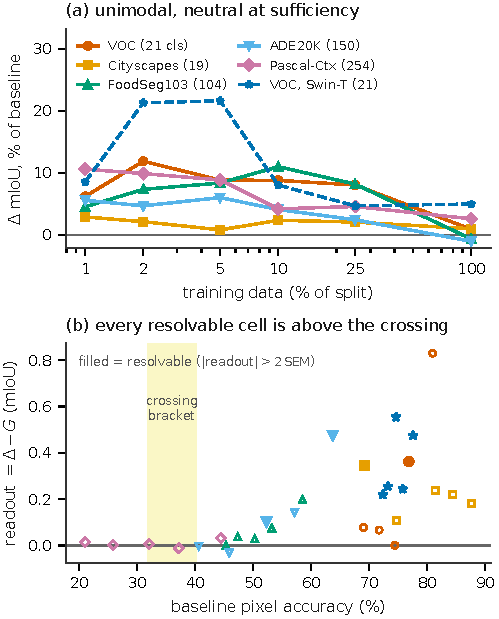
\includegraphics[width=\linewidth]{figs/dense_envelope.pdf}
\caption{Semantic segmentation, six populations, 200 epochs, three seeds per
cell. \textbf{(a)} $\Delta$ as a percentage of each cell's own baseline, not absolute mIoU, since the baselines differ eightfold. Read this way, four of
the six envelopes are unimodal, Cityscapes is flat within noise and
Pascal-Context is highest at $1\%$ and lower everywhere after; all six occupy
the same \denseRelLo--\denseRelHi\% band classification does across
$1$--$25\%$, and three go neutral or
negative at full data. \textbf{(b)} The \readout{} term against the head's own classification scale
(pixel accuracy), not mIoU: the crossing bracket is an accuracy bracket, and
scoring the law on mIoU puts every dense cell on the wrong flank. Filled
markers are the resolvable cells; all sit above the bracket, so segmentation
confirms the law's positive branch and cannot test its negative one.}
\label{fig:dense}
\end{figure}


Pascal-Context is the control that carries most of the weight: it re-annotates
the \emph{identical} VOC images at 254 classes instead of 21, so it separates a
label-space effect from a pixel effect exactly as CIFAR-100-super does on the
classification side.

\paragraph{Two measurement decisions, both of which we got wrong first.}
Absolute mIoU is not comparable across these populations: their baselines
differ eightfold ($51.5$ on VOC at full data, $6.4$ on Pascal-Context).
Comparing raw $\Delta$ across them makes the label-space effect look like a
collapse, more than $10\times$ in the mid band in absolute terms, when in
relative terms it is at most $2.3\times$, and runs
the other way at $1\%$ and $100\%$. We report both, and read comparisons off
the relative column.

Second, and more consequential: \emph{readout must be evaluated on the head's
own classification scale, not on mIoU.} The crossing bracket $[31.8, 40.3]$ was
measured in accuracy. mIoU is a far harsher statistic: it averages per-class
IoU with equal weight, so classes the model never learns dominate it, and a
cell at $6.2$ mIoU may be classifying $69\%$ of its pixels correctly. Scoring
the law on mIoU places every dense cell deep on the left flank and predicts a
negative \readout{} everywhere; scoring it on pixel accuracy places them on the
decayed positive branch, which is where they are. We registered this limitation
in advance and then violated it in our own prediction, which is how it was
found.

\begin{table}[pos=htbp]
\caption{The dense envelope. $\Delta$ in mIoU points, with $\Delta$ as a
percentage of that cell's own baseline beneath it. Three seeds per cell,
ResNet-18 with an FCN head at output stride 8, 200 epochs at every fraction,
the same budget the classification recipe uses. Pascal-Context is VOC's own
pixels relabelled to 254 classes. The last block ($\dagger$) is a Swin-Tiny encoder and is
a \emph{diagnostic} row, not a headline one: it trains under AdamW, not the frozen recipe, for the reason given in Sec.~\ref{sec:denseattn}, and
carries the bistability caveat that attaches to every Swin cell.}
\label{tab:dense}
\centering\scriptsize
\setlength{\tabcolsep}{3.0pt}
\zebra{2}
\begin{tabular}{lrrrrrrr}
\toprule
Population & Cls. & 1\% & 2\% & 5\% & 10\% & 25\% & 100\% \\
\midrule
VOC           & 21  & $+0.39$ & $+0.97$ & $+1.15$ & $+1.61$ & $+2.34$ & $+0.46$ \\
\quad rel.    &     & 6\%     & 12\%    & 9\%     & 9\%     & 8\%     & 1\%     \\
Cityscapes    & 19  & $+0.49$ & $+0.41$ & $+0.20$ & $+0.68$ & $+0.73$ & $+0.48$ \\
FoodSeg103    & 104 & $+0.12$ & $+0.20$ & $+0.26$ & $+0.43$ & $+0.56$ & $-0.12$ \\
ADE20K        & 150 & $+0.18$ & $+0.20$ & $+0.38$ & $+0.38$ & $+0.37$ & $-0.29$ \\
Pascal-Ctx    & 254 & $+0.11$ & $+0.13$ & $+0.16$ & $+0.10$ & $+0.16$ & $+0.17$ \\
\quad rel.    &     & 11\%    & 10\%    & 9\%     & 4\%     & 5\%     & 3\%     \\
\midrule
Swin-Tiny, VOC$^{\dagger}$ & 21 & $+0.42$ & $+1.29$ & $+1.76$ & $+0.90$ & $+0.75$ & $+1.31$ \\
\quad rel.    &     & 9\%     & 21\%    & 22\%    & 8\%     & 5\%     & 5\%     \\
\bottomrule
\end{tabular}
\end{table}

\subsection{Target--task alignment is not where the value comes
from}\label{sec:densealign} This is the section's main result and it is a
negative one. VOC at $1\%$ is 107 images over 20 classes, about five per class,
the same supervision density at which classification shows a universal
${\approx}+1.5$ floor (CIFAR-100 $+1.42$, Tiny-ImageNet $+1.49$). Dense
prediction at that density returns \textbf{$+\denseVocOneDelta$ mIoU}
(\denseVocOneRel\%), and the frozen-feature probe agrees ($G = +0.31$), so it
is not a \readout{} artifact.

So the venue built to flatter the prior, a dense target supervising a dense
task, pays \emph{less}, not more. Whatever the prior supplies, it is not
"structure that happens to match the output space." That makes the mechanism
claim in Sec.~\ref{sec:fusion} more precise, not weaker: the prior injects
oriented-energy structure into the representation, and what the head does with
it afterwards is a separate question.

\subsection{The regimes transfer; the magnitudes are metric-bound}
In absolute mIoU the dense gains look tiny beside the classification ones. In
relative terms they run \denseRelLo--\denseRelHi\% of baseline across the
$1$--$25\%$ band (three populations go negative at $100\%$, to $-1.1\%$),
which is the
range classification occupies (CIFAR-100 at $5\%$ is $+5.15$ on $25.36$, i.e.\
$20\%$). The shape transfers on four of the six populations, and we give the
other two instead of averaging them away: reading the relative column
throughout, VOC peaks at $2\%$ and FoodSeg103 at $10\%$ (in absolute mIoU both
instead peak at $25\%$, VOC at $+\denseVocPeak$) and ADE20K at $5\%$, while
Cityscapes is flat within noise, dipping
at $5\%$ and rising again, and Pascal-Context falls from $1\%$ with one
uptick between $10$ and $25\%$.
ADE20K's absolute column would instead put its peak at $10\%$, but the two
candidate cells differ by $0.006$ mIoU against standard errors of $0.02$ and
$0.15$, so that location is unresolvable and we do not assert it.

At full data the gain decays to neutrality or below on three of the six (VOC
$+\denseVocFull$, i.e.\ \denseVocFullRel\%; FoodSeg $-0.12$; ADE20K $-0.29$),
and stays positive on Cityscapes ($+0.48$, though indistinguishable from
VOC's $+\denseVocFull$), Pascal-Context ($+0.17$, resolved
at ten standard errors) and Swin-VOC ($+1.31$). Structural neutrality at
sufficiency therefore holds on the three populations large enough to reach
sufficiency, and the exceptions are the ones this study's own image-count axis
predicts: Cityscapes trains on $2{,}975$ images and Pascal-Context on
$4{,}998$, which are low-data cells here whatever their label says, exactly as
DTD and CUB-200 are in the classification grid.

\paragraph{A validity note that changed a conclusion.} We first ran this grid
at 50 epochs and reported an envelope that was monotone rising on every
population, with no right flank. That was an artifact. At 200 epochs the VOC
$10\%$ baseline rises from $7.23$ to $18.28$ mIoU ($+153\%$), and the 50-epoch
curves were still climbing at ${\sim}0.7$ mIoU/epoch when the cosine schedule
annealed the step size away. Their apparent convergence was the schedule, not
the model. Re-pinning the dense recipe to 200 epochs, matching the
classification budget instead of choosing one to suit the task, moved
$\Delta(\mathrm{VOC},100\%)$ from $+2.57$ to $+0.46$, i.e.\ from a nominal
falsification of neutrality at sufficiency to a confirmation of it: an
under-trained instrument did not merely add noise here, it produced the
opposite answer twice (Sec.~\ref{sec:dataopt}).

\subsection{The law on a different task and a different metric}
Of the \denseLawCells{} cells carrying both $\Delta$ and $G$ (full-data cells
are excluded: there the probe's labels \emph{are} the cell's labels, so no
split is interpretable), \denseLawBracket{} sit inside the crossing bracket
where the law makes no sign call and \denseLawUnres{} have $|\readout|
\leq 2$\,SEM, which on the right flank is expected, not disappointing: $\Delta$
and $G$ are both near zero there and the sign of their difference is noise.
That leaves \denseLawResolvable{} cells that actually test the law, and
\denseLawCorrect{} of \denseLawResolvable{} fall on the predicted side.

\looseness=-1 The qualification is that all \denseLawResolvable{} sit
\emph{above} the crossing (pixel accuracy \denseLawPixLo--\denseLawPixHi), so
segmentation confirms the law's positive branch on a new task and a new metric
and does not test its negative branch. Pascal-Context was built to supply
exactly that test, and the reason it cannot is worth stating before its numbers
rather than after them: resolving a \readout{} requires not only a baseline below
the bracket but a $\Delta$ large enough that $\Delta - G$ exceeds its own
uncertainty, and Pascal-Context's $\Delta$ runs $+0.10$ to $+0.17$ mIoU.
The \readout{} there is a difference between two small numbers whatever its sign. What
it delivers is therefore a null by construction: trained pixel accuracy $21.1$
and $25.9$ at $1$--$2\%$, clearly below the bracket where a negative \readout{} is
required, and a \readout{} of $+0.02$ and $+0.00$, zero, not negative. The
pre-registered falsifier needed a clearly positive \readout{} and did not fire;
the prediction was not confirmed either; we record the cells as
\emph{unresolved} and claim nothing from them. A population that could settle
it needs abundant labels, low pixel accuracy \emph{and} a material $\Delta$ at
once, and none of our six has all three.

\subsection{Attention, narrowed}\label{sec:denseattn}
On classification the prior is worth roughly twice as much to a
hierarchical-attention backbone as to a convolutional one ($G_{\mathrm{swin}} =
7.6$--$10.5$ against $G_{\mathrm{r18}} = 3.55$--$6.26$ on CIFAR-100). On dense
prediction that advantage survives only in a narrow band. Relative feature
gain, Swin against ResNet-18 on identical images: $4.6$, $20.7$, $17.5$, $7.0$,
$2.0\%$ at $1$--$25\%$, against $6.3$, $13.4$, $10.8$, $8.1$, $5.8\%$. Swin
leads at $2\%$ and $5\%$ by ${\sim}1.6\times$ and trails at $1\%$, $10\%$ and
$25\%$; by $25\%$ its $G$ has collapsed to $+0.27$ against convolution's
$+1.51$. At full data it still gains ($+1.31$, $5\%$ relative) where the
convolutional arm is near-neutral ($+0.46$, $1\%$), which does mirror the
classification result.

We state this narrowly on purpose. An earlier, under-trained version of this
experiment supported the opposite conclusion, that the attention deficit does
not transfer to dense prediction, and a four-fraction reading of the corrected
data supported a broader one. Both were over-readings of the fractions then
available. Swin is not ViT, this is one dataset, and these are AdamW diagnostic
cells; what they establish is that the attention advantage is task- and
regime-dependent, not that it is absent.

\subsection{The label-space effect is much weaker than it looks}
VOC and Pascal-Context are byte-identical pixels at 21 and 254 classes. In
absolute mIoU the gap is large at every fraction, and at full data VOC's
$+\denseVocFull$ against Pascal-Context's $+\densePcFull$ invites a conclusion
about label granularity. Normalized, it mostly disappears: \denseVocFullRel\%
against \densePcFullRel\% at full data, $9\%$ against $9\%$ at $5\%$, and
Pascal-Context is \emph{higher} at $1\%$ ($11\%$ against $6\%$). Relative
feature gain behaves the same way. The defensible statement is a mid-band
tendency for the coarser label space, not the collapse the absolute numbers
suggest, and it is visible as such only because the control holds the pixels
fixed.

\subsection{Detection: the prior does not reach a coordinate
regressor}\label{sec:detection} Segmentation still asks a network to
\emph{label}, one decision per pixel. Detection is the only task here whose
head \emph{regresses coordinates}, and oriented energy is about edges and
extents, so if the prior were going to help anything localize this is where it
would show. We run it on the same VOC images and the same committed subset
indices the segmentation cells use, with the dense recipe verbatim (200 epochs,
identical crops and augmentation) and a single-level anchor-free FCOS head at
stride 8 on the same tapped backbone. Detection therefore differs from
segmentation in the head and the loss and in nothing else. \detCells{} runs
(\detCellCount{} cells in the sense of Sec.~\ref{sec:stats}): six fractions,
both arms, three seeds.

\begin{table}[pos=htbp]
\caption{Detection is a null. $\Delta$ is aux minus baseline on PASCAL VOC.
AP50 is the task metric; fg\_acc and fg\_iou are the head's 20-way accuracy and
its mean box IoU \emph{at ground-truth foreground locations}, so neither can
collapse the way a ranked-precision integral does. $G$ is the same quantity
under a frozen trunk with a fresh $1\times1$ head fitted on the full split.
Cells marked $\dagger$ (\detFloorPcts) fall under the pre-declared floor rule:
both arms below 1.0 AP50, where a difference is not a measurement.}
\label{tab:det}
\centering\scriptsize
\setlength{\tabcolsep}{3.6pt}
\zebra{2}
\begin{tabular}{lrrrrr}
\toprule
Data & $\Delta$AP50 & $\Delta$fg\_acc & $\Delta$fg\_iou & $G$(fg\_acc) & $G$(fg\_iou) \\
\midrule
1\%$^\dagger$  & $\detOneDelta$ & $-0.23$ & $-0.0003$ & $-0.16$ & $+0.0017$ \\
2\%$^\dagger$  & $-0.00$ & $-0.23$ & $-0.0001$ & $-0.37$ & $-0.0006$ \\
5\%            & $-0.08$ & $+0.11$ & $-0.0048$ & $+0.34$ & $+0.0130$ \\
10\%           & $+0.56$ & $-0.32$ & $+0.0032$ & $+0.08$ & $+0.0073$ \\
25\%           & $-0.41$ & $+0.01$ & $+0.0017$ & $-0.47$ & $+0.0011$ \\
100\%          & $\detFullDelta$ & $+0.64$ & $+0.0031$ & --      & --        \\
\bottomrule
\end{tabular}
\end{table}

\paragraph{The result, and one number that was not real.} Every measure is flat
(Table~\ref{tab:det}). The single exception is $+\detTenDelta$ AP50 at 10\%,
and we do not report it as a gain: its own components are all consistent with
zero ($\Delta$fg\_acc $-0.32$, $\Delta$fg\_iou $+0.0032$), and at AP25 it
falls to $+0.35$, inside noise. A gain that is neither classification nor
localization and does not survive a threshold change is ranking noise.

We also had to withdraw a larger number. At 5\% the raw arithmetic gives
$+0.81$ AP50, and it is entirely one collapsed baseline seed: its fg\_iou is
\emph{exactly} $0.0000$ while its fg\_acc matches its siblings, and its
regression loss pins at exactly $1.0000$ from epoch 29 to 199. The predicted
boxes went to zero area, the GIoU term saturated, its gradient vanished, and
that branch could never recover while the classification branch kept improving.
This is a \emph{partial} collapse of one branch of a two-headed model, and the
seed-level check used elsewhere in this study would not have caught it, because
the cell still trains. Excluding it, $\Delta$ at 5\% is $-0.08$.

\paragraph{The null is the prior, not the head.} A flat end-to-end result on a
task with a weak head admits a second reading, and it is the one this study
documents everywhere else: at five images per class the frozen-feature probe on
CIFAR-100 sees $+4.82$ of feature gain where the trained classifier realizes
$+1.87$. So we probed the detection trunks under the same protocol, and the
answer is unambiguous: $G(\mathrm{fg\_acc}) = \detOneGFgAcc$ at 1\% and $-0.37$
at 2\%, against a pre-registered falsifier at $+1.5$. A fresh head with a
hundred times the cell's labels extracts nothing more from the prior's trunk
than from the baseline's.

What licenses that reading is that the probe demonstrably works here: at 1\% it
lifts fg\_acc from the trained cell's \detOneFgAcc{} to \detProbeLiftOne. The
trained detection head really is label-limited at 107 images, which is exactly
the condition under which the classification left flank hides feature gain. The
condition is met and there is nothing to find. One quantity does move,
$G(\mathrm{fg\_iou}) = +\detTenGFgIou \pm \detTenGFgIouSem$ at 10\%, resolvable
and localization-side, not classification-side, but $0.007$ of IoU is not a
result we will build on.

\paragraph{Two things this cannot be blamed on.} The instrument is adequate: at
full data the detector reaches \detFullAPnone{} AP50 from scratch, so the null
is not a broken head, and the recorded multi-level-FPN conditional does not
reopen. And the recipe is the
segmentation recipe unchanged, on the same images, so this is not the
undertrained-instrument error of the 50-epoch dense grid.

\paragraph{What detection cannot do, stated as a limitation.} We had hoped it
would supply the negative branch of the sign law, which segmentation could not:
baseline fg\_acc is $\detOneFgAcc$--$28.9$ at 1--5\%, below the crossing
bracket, and $\Delta \approx 0$ there, so $\readout = -G$. It does not,
and the obstruction is structural. The law needs $G$ on the \emph{same} metric
as $\Delta$, and the probe's own AP50 floors at $1$--$2\%$ ($\detProbeOneAP$ at 1\%) and
sits at the floor's edge at $5\%$ ($0.97$ and $1.15$ on the two arms). Above the crossing $\Delta$ and $G$ are both near
zero, so their difference is unresolvable. Detection contributes no resolvable
law cell, the same outcome as Pascal-Context and for the same reason. The
negative branch remains untested by either non-classification task, and we
prefer to say so rather than construct a fifth instrument to chase it.

\paragraph{The task axis.} Taken with Sec.~\ref{sec:densealign}, the three
tasks order cleanly and the ordering is the sharpest limit we can put on the
method: what the prior supplies is realized \emph{fully} by a whole-image
classifier, \emph{partly} by a per-pixel classifier, and \emph{not at all} by a
coordinate regressor. In the last case we now know why: the features are not
there, not the head being unable to reach them.
